% mainfile: ../../../../master.tex
\subsection{Configuring AOSP for Acme Device on Ubuntu 23}
\label{task:20231118_aosp_hal}

% The interface to the hardware is a device drivers which are usually device specific and sometimes proprietary. A single set of C header files describes the functionality that a HAL provides to the Android system. HAL Code for a particular device is the implementation of the API defined by those header files, so that no code above the HAL needs to be changed to port Android to use the new device.

\subsubsection*{Repo Manifest}

Top-level subdirectory named \path{.repo} contains the \path{manifests} repository inside \path{manifests} subdirectory. The \path{manifests} repo contain one or more manifest files named as the argument of the \path{-m} command line option. \path{.repo/manifest} file controls the structure of the rest of the repository, and includes \path{.repo/manifests/default.xml}\footnote{\url{https://gerrit.googlesource.com/git-repo/+/master/docs/manifest-format.md}} which is a list of git repositories. \path{repo} program parses \path{manifest.xml}, and thus \path{default.xml}, and clone each repository into a location specfied inside \path{default.xml}.

Each \path{project} element in the XML identifies a git repository by its \path{name}, relative to some base URL, its \path{remote}; and where that repository should be placed in the local workspace, its \path{path}. If the full URL for the repository is not specified, repo will use the default remote specified in the \path{default} element near the top of the manifest:
\begin{lstlisting}[language=xml]
<default revision="refs/tags/android-13.0.0_r11"
    remote="aosp"
    sync-j="4" />
\end{lstlisting}
where the remote, \path{aosp}, is defined likewise in the top of of the \path{default.xml}:
\begin{lstlisting}[language=xml]
<remote  name="aosp"
    fetch=".."
    review="https://android-review.googlesource.com/" />
\end{lstlisting}
Instead of including a URL as its attribute, it includes the \path{fetch} attribute which indicatese the URL for this remote should be derived from the URL used to initialize the workspace (the argument to the \path{-u} option).


\begin{lstlisting}
git ls-remote -h https://android.googlesource.com/platform/manifest.git
repo init -u https://android.googlesource.com/platform/manifest -b android-10.0.0_r33
git config --global user.email "mg.weiminn@gmail.com"
git config --global user.name "weiminn"
repo init -u https://android.googlesource.com/platform/manifest -b android-10.0.0_r33
repo sync -j31
source build/envsetup.sh 
lunch sdk_phone_x86_64-userdebug 
make -j31
\end{lstlisting}
% sudo apt-get install libncurses-dev

Ubuntu $23$ does not have the repository for \path{libncurses5} because they already have \path{libncurses6}, so you have to add old \path{focal} repository to your \path{/etc/apt/sources.list}:
\begin{lstlisting}[language=bash]
deb http://security.ubuntu.com/ubuntu focal-security main universe
\end{lstlisting}

After including the old repo, update the repository index and install \path{libncurses5}: 
\begin{lstlisting}[language=bash]
sudo apt update
sudo apt install libncurses5
\end{lstlisting}

% \begin{figure}[H]
%     \centering
%     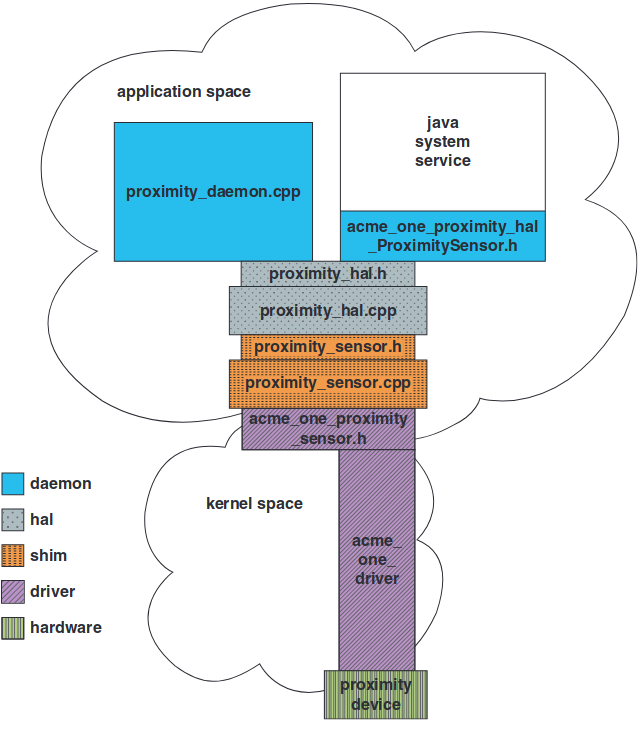
\includegraphics[width=.75\linewidth]{entries/2023/11/17/hal.png}
%     \caption{HAL Layer Structure}
%     \label{fig:hallayerstruct}
% \end{figure}

